\documentclass[11pt]{article}

\usepackage[margin=1in]{geometry}
\usepackage{amsmath,amssymb,amsthm}
\usepackage{graphicx}
\usepackage{booktabs}
\usepackage{xcolor}
\usepackage[numbers,sort&compress]{natbib}
\usepackage[colorlinks=true,linkcolor=black,citecolor=blue,urlcolor=blue]{hyperref}

\graphicspath{{figures/}}
\setlength{\emergencystretch}{2em}  % absorb the few tight lines cleanly
\newcommand{\wfer}{\mathrm{WFER}}
\newcommand{\srtrue}{\mathrm{SR}_{\mathrm{true}}}
\newcommand{\srfwd}{\mathrm{SR}_{\mathrm{fwd}}}

\title{\bfseries Does Walk-Forward Validation Predict\\ Out-of-Sample Performance?\\
A Controlled Study of the Walk-Forward\\ Efficiency Ratio and Window Design}

\author{Eugen Soloviov\thanks{Independent Researcher. ORCID:
\href{https://orcid.org/0009-0006-3148-111X}{0009-0006-3148-111X}.
Correspondence: \href{mailto:suenot@gmail.com}{suenot@gmail.com}.
Code to reproduce every number and figure:
\url{https://github.com/suenot/wfo-validity}.}}

\date{}

\begin{document}
\maketitle

\begin{abstract}
Walk-forward optimization is the de facto validation protocol of systematic
trading, and the \emph{walk-forward efficiency ratio} (WFER)---out-of-sample
(OOS) performance over in-sample (IS) performance---is its de facto acceptance
statistic, graded in practitioner folklore as excellent above $0.8$, acceptable
above $0.5$, and overfit below $0.3$--$0.5$. To our knowledge neither the ratio
nor the grading has ever been measured against a known ground truth. We build a
controlled simulation in which a one-parameter strategy family has a known,
time-varying annualized-Sharpe surface---stationary, drifting optimum,
structural break, or no-edge null---so the true forward Sharpe of every
deployed configuration is computable exactly, and we run five validation
procedures (single split, anchored and rolling walk-forward, naive shuffled
$k$-fold, and a CPCV-lite) on the same $8{,}000$ simulated histories
($2{,}000$ per regime), plus a $9{,}000$-run window-design sweep. The verdict
is mixed. WFER carries real signal: the per-period normalized ratio correlates
with true forward Sharpe at Spearman $+0.45$ and detects deployed losers at
AUC $0.74$. But it is dominated by simpler statistics computed from the same
folds---the stitched OOS $t$-statistic reaches AUC $0.78$ and the stitched OOS
Sharpe $\rho\,{+}0.53$---so the ratio's distinguishing step, dividing by IS
PnL, only adds noise. The folk thresholds are miscalibrated: runs with
$\wfer\ge 0.8$ do no better forward than runs at $0.5$--$0.8$ (mean forward
Sharpe $+0.98$ vs.\ $+0.99$), the ``borderline/overfit'' zone below $0.5$
contains configurations averaging $+0.59$ to $+0.83$, and the literal raw-PnL
ratio---which compares accumulation windows of different lengths---reaches
$0.5$ in only $6$ of $8{,}000$ runs, so the thresholds are essentially
unreachable under the formula that usually accompanies them. The per-window
ratio is ill-conditioned in $21\%$ of runs ($47\%$ under the null), where
near-zero IS denominators make single-window readings arbitrarily wild.
Window folklore fares partly better. Anchored walk-forward beats rolling under
stationarity ($+0.10$ forward Sharpe, $p\approx 2\times10^{-39}$) and rolling
beats anchored under drift ($+0.08$) and breaks ($+0.15$): the advertised
direction, with an unadvertised stationarity price. Window length matters
mainly for the \emph{estimate}, not the deployment: the WFER--forward rank
correlation peaks at $0.52$ near nine folds and collapses to $0.23$ at one
fold, while deployed performance is flat for train windows of $126$ periods or
more. Across procedures, rolling deploys best (mean forward Sharpe $0.66$
vs.\ $0.62$ for anchored, CPCV-lite, and $k$-fold, $0.56$ for a single split);
naive shuffled $k$-fold is the most optimistic estimator ($+0.08$ Sharpe bias,
worse under drift and breaks); CPCV-lite's estimate ranks outcomes best
($\rho\,0.64$). In short: WFER is informative but redundant; its thresholds
are folklore and miscalibrated; the window-design advice is directionally
right and incompletely priced.
\end{abstract}

\section{Introduction}

The standard validation ritual of systematic trading is
\emph{walk-forward optimization} (WFO): optimize the strategy's parameters on
an in-sample (IS) window, evaluate the selected configuration on the
immediately following out-of-sample (OOS) segment, roll the window forward,
and stitch the OOS segments into a single pseudo-live track record
\citep{pardo1992design,pardo2008evaluation,tomasini2009trading}. Its
acceptance statistic is the \emph{walk-forward efficiency} of
\citet{pardo2008evaluation}: the ratio of OOS to IS performance, near one when
the optimization captured persistent structure and near zero when it
curve-fit noise. The statistic is embedded in commercial
tooling---TradeStation's Walk-Forward Optimizer fails any strategy whose
walk-forward efficiency falls below $50\%$
\citep{tradestation_wfo}---and around it has
grown an informal grading folklore: ratios above ${\sim}0.8$ signal
robustness, $0.5$ marks the pass/fail boundary, and values below
${\sim}0.3$ indicate overfitting. In circulating recipes the ratio is often
computed literally as summed OOS PnL over summed IS PnL, and read both in
aggregate and window by window.\footnote{The literal raw-PnL WFER recipe and
the $0.8/0.5/0.3$ grading table tested in this paper appear in the author's
own earlier practitioner writing (a market-making blog post on walk-forward
optimization). This paper is therefore a controlled self-audit of advice the
author has himself circulated, not an attack on a third party. The thresholds
have no citable primary source that we could locate; the only stable
documented artifact is TradeStation's WFE $\ge 50\%$ pass criterion
\citep{tradestation_wfo}, and we deliberately do not attribute the triple to
\citet{pardo2008evaluation}.}

None of this folklore has, to our knowledge, been measured where the truth is
known. Does the walk-forward efficiency ratio (WFER) actually predict forward
performance---and better than what alternative? Do the thresholds correspond
to calibrated decision boundaries? Should the IS window be anchored
(expanding) or rolling, and how finely should the history be partitioned into
folds? The academic literature rigorously treats adjacent problems---backtest
overfitting \citep{bailey2014pseudomathematics,bailey2017probability},
data snooping \citep{white2000reality}, splitting schemes for dependent data
\citep{bergmeir2012use,lopezdeprado2018advances}---but the WFE ratio itself,
the statistic practitioners actually gate deployments on, has remained
untested.

We provide that test in a controlled simulation. A one-parameter strategy
family has a population annualized-Sharpe surface that we control exactly,
including how its optimum moves through time: it can stay put (stationary),
drift linearly, jump at a structural break, or not exist at all (a no-edge
null). Because the surface is known, the true expected Sharpe of deploying
\emph{any} configuration over a future horizon is computable exactly, and
every validation procedure---and every diagnostic it emits---can be judged
against that ground truth. Our findings are deliberately mixed: the ratio is
genuinely informative yet strictly dominated by simpler statistics computed
from the very same folds; its thresholds fail in two distinct ways; and the
window-design folklore is directionally right at an unstated price.

\paragraph{Contributions.}
\begin{enumerate}\itemsep2pt
\item A reproducible framework in which walk-forward validation is run against
a known, \emph{time-varying} Sharpe surface under four regimes (stationary,
drift, break, null), with five procedures evaluated on the same simulated
histories and the forward truth of every deployment computed exactly:
$8{,}000$ main experiments evaluating all five procedures, plus a
$9{,}000$-run window-design sweep of the rolling procedure
(Sections~\ref{sec:framework}--\ref{sec:setup}).
\item The first operating characteristics of the WFER. It carries signal
(Spearman $\rho=0.451$ against true forward Sharpe; AUC $0.743$ for detecting
deployed losers) but is dominated, on every regime with an edge, by the
stitched OOS $t$-statistic (AUC $0.781$) and OOS Sharpe ($\rho=0.529$)
computed from the same folds; and its per-window form is ill-conditioned in
$21.4\%$ of runs ($47.3\%$ under the null)
(Sections~\ref{sec:informative} and~\ref{sec:illcond}).
\item A calibration of the folk thresholds. The $\ge 0.8$ bin is
indistinguishable from $0.5$--$0.8$ (mean forward Sharpe $0.980$ vs.\
$0.994$); the ``borderline/overfit'' zone below $0.5$ contains configurations
averaging $+0.59$ to $+0.83$; and the literal raw-PnL ratio cannot reach its
own thresholds ($6$ of $8{,}000$ runs at ${\ge}0.5$), because it compares
accumulation windows of different lengths (Section~\ref{sec:thresholds}).
\item A paired anchored-vs.-rolling comparison on identical OOS segments:
anchored wins under stationarity ($+0.100$ forward Sharpe,
$p\approx2\times10^{-39}$), rolling under drift ($+0.079$) and breaks
($+0.154$)---the folklore direction, with a stationarity cost the folklore
does not state (Section~\ref{sec:avr}).
\item A window-design sweep and a five-procedure ranking showing that window
length shapes mainly the \emph{estimate} (diagnostic--forward correlation
peaks at $0.52$ near nine folds, collapses to $0.23$ at one fold), not the
deployment (flat for train length ${\ge}126$); that rolling WFO deploys best
($0.657$) while naive shuffled $k$-fold is the most optimistic estimator
($+0.083$ bias, worse under drift and breaks); and that CPCV-lite's estimate
ranks outcomes best ($\rho=0.636$)
(Sections~\ref{sec:window}--\ref{sec:ranking}).
\end{enumerate}

\section{Related work}
\label{sec:related}

\paragraph{Walk-forward optimization and the efficiency ratio.}
Walk-forward analysis originates in the practitioner literature on
trading-system development. \citet{pardo1992design} introduced the procedure
of repeatedly optimizing a strategy's parameters on an IS window and
evaluating the selected configuration on the immediately following OOS
segment, stitching the OOS segments into a single pseudo-live track record.
The substantially revised second edition \citep{pardo2008evaluation}
systematized the methodology and proposed the \emph{walk-forward efficiency}
(WFE)---the ratio of annualized OOS performance to annualized IS
performance---as the central diagnostic of whether an optimization captured
persistent structure or merely curve-fit noise. Practitioner texts adopted
the procedure essentially unchanged \citep{tomasini2009trading}, and it is now
embedded in retail and institutional tooling: TradeStation's Walk-Forward
Optimizer, for example, fails any strategy whose WFE falls below $50\%$ under
its default test criteria \citep{tradestation_wfo}. Around this default has
grown an informal grading folklore---ratios near $0.8$ signal robustness,
$0.5$ marks the pass/fail boundary, and values below roughly $0.3$ indicate
overfitting---that circulates in platform documentation, trading courses, and
blogs without any traceable empirical validation. To our knowledge, no
published study has measured the operating characteristics of the WFE ratio
(its sampling distribution, its correlation with true forward performance, or
the error rates implied by these thresholds) in a setting where the ground
truth is known. Nor has the practitioner literature resolved basic design
questions it raises only heuristically: anchored versus rolling in-sample
windows, and how finely the history should be partitioned into walk-forward
folds.

\paragraph{Backtest overfitting and multiple testing.}
A parallel academic literature has quantified how easily backtests mislead.
\citet{bailey2014pseudomathematics} showed that the expected maximum Sharpe
ratio over $N$ random configurations grows without bound, so impressive IS
results are nearly guaranteed given enough trials. \citet{bailey2017probability}
formalized the \emph{probability of backtest overfitting} (PBO) via
combinatorially symmetric cross-validation (CSCV), which evaluates whether
configurations selected in-sample systematically underperform out-of-sample.
\citet{bailey2014deflated} derived the deflated Sharpe ratio, which corrects
observed performance for the number of trials and non-normality, and
\citet{harvey2015backtesting} proposed multiple-testing haircuts to reported
Sharpe ratios; \citet{arnott2019backtesting} distilled these concerns into a
research protocol for the machine-learning era. This line of work descends
from the data-snooping literature in econometrics: \citet{white2000reality}
introduced the Reality Check for testing whether the best of many models
beats a benchmark after accounting for the search, and \citet{hansen2005test}
sharpened it into the more powerful Superior Predictive Ability test. These
tools diagnose selection bias \emph{given} a backtesting protocol; they do not
tell us whether walk-forward validation itself---the protocol practitioners
actually use to combat overfitting---produces forward-performance estimates
that can be trusted, nor how its diagnostic ratio behaves under regime change.

\paragraph{Cross-validation for dependent data.}
A third strand asks how predictive accuracy should be estimated for time
series at all. \citet{tashman2000outofsample} reviewed out-of-sample
evaluation designs---fixed versus rolling origins, window updating, single
versus multiple test periods---and noted how sensitive conclusions are to
these choices. \citet{bergmeir2012use} compared blocked and standard
cross-validation against last-block evaluation for machine-learning
predictors, finding cross-validation often yields more robust model
selection; \citet{bergmeir2018note} proved that standard $k$-fold
cross-validation remains valid for purely autoregressive models with
uncorrelated errors. Conversely, \citet{cerqueira2020evaluating} found
empirically that out-of-sample (forward) procedures are more reliable than
cross-validation when series are non-stationary. In finance,
\citet{lopezdeprado2018advances} argued that naive $k$-fold leaks information
through overlapping and serially correlated labels, proposing purged $k$-fold
and combinatorial purged cross-validation (CPCV) as alternatives that
generate many backtest paths. This debate concerns \emph{splitting schemes}
and the bias of error estimates; the WFE ratio---a statistic computed on top
of a splitting scheme and an optimization step---has remained outside its
scope.

\paragraph{In-sample versus out-of-sample tests and window choice.}
Econometricians have long questioned the primacy of OOS evidence.
\citet{inoue2005insample} showed that in-sample and out-of-sample
predictability tests are equally reliable under the null, and that
sample-splitting sacrifices power, so insisting on OOS confirmation is not a
free lunch. \citet{rossi2012outofsample} demonstrated that OOS conclusions
can hinge on the arbitrary choice of estimation-window size and proposed
tests robust to that choice, while \citet{inoue2017rolling} derived optimal
rolling-window sizes when parameters drift---directly relevant to the
anchored-versus-rolling question in walk-forward design. The survey of
\citet{rossi2013exchange} documents pervasive model instability as a central
fact of predictive finance. These results imply that walk-forward outcomes
are functions of window design in ways practitioners rarely acknowledge, but
the literature evaluates forecast accuracy tests, not parameter-selection
pipelines with a WFE-style acceptance rule.

\paragraph{Positioning.}
In sum, walk-forward optimization is the de facto standard validation
protocol in systematic trading, and the walk-forward efficiency ratio is its
de facto acceptance statistic---yet both live almost entirely in practitioner
folklore. The academic literature offers rigorous tools for adjacent
problems: detecting data snooping \citep{white2000reality,hansen2005test},
quantifying backtest overfitting
\citep{bailey2017probability,bailey2014deflated}, and choosing splitting
schemes for dependent data
\citep{bergmeir2012use,lopezdeprado2018advances,cerqueira2020evaluating}.
None of it validates the WFE ratio against a known ground truth, tests the
$0.8/0.5/0.3$ folk thresholds, or compares anchored and rolling walk-forward
against purged cross-validation under controlled stationarity, drift, and
structural breaks. This paper fills that gap with a simulation study in which
the true, time-varying Sharpe surface is known by construction, so the
predictive value of every diagnostic can be measured exactly.

\section{The efficiency ratio and the validation procedures}
\label{sec:wfer}

\paragraph{Setting.} A strategy family is indexed by a parameter
$\theta$ on a grid in $[0,1]$. A validation procedure partitions a history of
$T_{\mathrm{hist}}$ periods into folds $j=1,\dots,J$, each with a train
window $W_j^{\mathrm{tr}}$ and a test window $W_j^{\mathrm{te}}$. Within each
fold the selection rule is fixed throughout this paper:
$\hat\theta_j = \arg\max_\theta \widehat{\mathrm{SR}}(\theta;
W_j^{\mathrm{tr}})$, the argmax of the annualized train-window Sharpe. Let
$I_j$ and $O_j$ be the summed PnL of $\hat\theta_j$ over
$W_j^{\mathrm{tr}}$ and $W_j^{\mathrm{te}}$, and let
$N_{\mathrm{IS}}=\sum_j |W_j^{\mathrm{tr}}|$,
$N_{\mathrm{OOS}}=\sum_j |W_j^{\mathrm{te}}|$.

\paragraph{Two readings of the ratio.} The literal practitioner formula is the
\emph{raw} ratio of PnL sums,
\begin{equation}
\wfer_{\mathrm{raw}} \;=\; \frac{\sum_j O_j}{\sum_j I_j},
\label{eq:raw}
\end{equation}
while Pardo's annualized-to-annualized definition corresponds to the
\emph{per-period normalized} form
\begin{equation}
\wfer_{\mathrm{norm}} \;=\;
\frac{\sum_j O_j / N_{\mathrm{OOS}}}{\sum_j I_j / N_{\mathrm{IS}}}
\;=\; \frac{N_{\mathrm{IS}}}{N_{\mathrm{OOS}}}\,\wfer_{\mathrm{raw}}.
\label{eq:norm}
\end{equation}
The distinction is not cosmetic. In walk-forward practice the IS windows are
several times longer than the OOS windows (three to four times in our
designs), so \eqref{eq:raw} divides PnL accumulated over very different
amounts of time: even a perfectly persistent edge scores
$\wfer_{\mathrm{raw}} \approx N_{\mathrm{OOS}}/N_{\mathrm{IS}} \approx
0.25$--$0.33$. The normalized form \eqref{eq:norm} is the only reading under
which the folk thresholds ($\ge 0.8$ ``excellent,'' $0.5$--$0.8$
``acceptable,'' $0.3$--$0.5$ ``borderline,'' $<0.3$ ``overfit,'' $<0$
``unprofitable'') can even potentially be meaningful; Section~\ref{sec:thresholds}
quantifies what happens when they are applied to either form. Both forms are
undefined when $\sum_j I_j \le 0$ (the implicit assumption of the grading
table is a positive IS denominator), and the per-window variant $O_j/I_j$ is
ill-conditioned whenever a single $I_j$ is near zero
(Section~\ref{sec:illcond}).

\paragraph{Five procedures.} We evaluate five ways of building the folds, all
sharing the selection rule above (Figure~\ref{fig:setup}, bottom):
\begin{itemize}\itemsep2pt
\item \textbf{Single split}: one fold; the last $25$--$35\%$ of the history is
held out. Deploys the argmax of the train portion.
\item \textbf{Anchored WFO}: expanding train window from the start of history;
aligned OOS segments of length $L_{\mathrm{test}}$ starting at
$L_{\mathrm{train}}$. Deploys the argmax over the full history (its last
expanding window, extended to the end).
\item \textbf{Rolling WFO}: train window of fixed length $L_{\mathrm{train}}$
ending where each OOS segment begins; the step equals $L_{\mathrm{test}}$, so
OOS segments tile the history without overlap and anchored/rolling share
\emph{identical} test segments---their comparison is paired on the same data.
Deploys the argmax over the most recent $L_{\mathrm{train}}$ periods.
\item \textbf{Naive shuffled $k$-fold}: the deliberately time-blind baseline;
$k=5$ shuffled folds. Deploys the textbook CV selection: argmax of the mean
per-fold test Sharpe.
\item \textbf{CPCV-lite}: a documented simplification of combinatorial purged
cross-validation \citep{lopezdeprado2018advances}: the history is cut into
$6$ contiguous groups, every $\binom{6}{2}=15$ choice of $2$ test groups
forms a fold, and an embargo of $10$ periods is dropped from the train set at
each test-group boundary. We call it ``lite'' deliberately: in our generative
model returns are serially independent given the surface, so there are no
overlapping labels to purge; the embargo mirrors the procedure as practiced
rather than removing genuine leakage. (CPCV is distinct from the CSCV scheme
of \citet{bailey2017probability}, which underlies PBO.) Deploys the argmax
over the full history, per the final-fit convention.
\end{itemize}

\paragraph{Diagnostics.} From each procedure's folds we record the two WFER
variants \eqref{eq:raw}--\eqref{eq:norm} and five simpler statistics computed
from the same raw material: the \emph{stitched OOS Sharpe} (annualized Sharpe
of the concatenated test-window returns of the per-fold selections), the
\emph{OOS $t$-statistic} ($\bar r_{\mathrm{OOS}}/s_{\mathrm{OOS}}\cdot
\sqrt{N_{\mathrm{OOS}}}$), the mean per-fold \emph{IS$\to$OOS rank
correlation} (Spearman correlation across $\theta$ between train-window and
test-window Sharpe), the \emph{fold win rate} (fraction of folds with
$O_j>0$), and the \emph{$\theta$-instability} (standard deviation of the
selected $\hat\theta_j$ across folds, in $[0,1]$ units; the folklore reads
unstable selections as a warning sign, so it enters orientation-flipped).

\section{Simulation framework}
\label{sec:framework}

\begin{figure}[t]
\centering
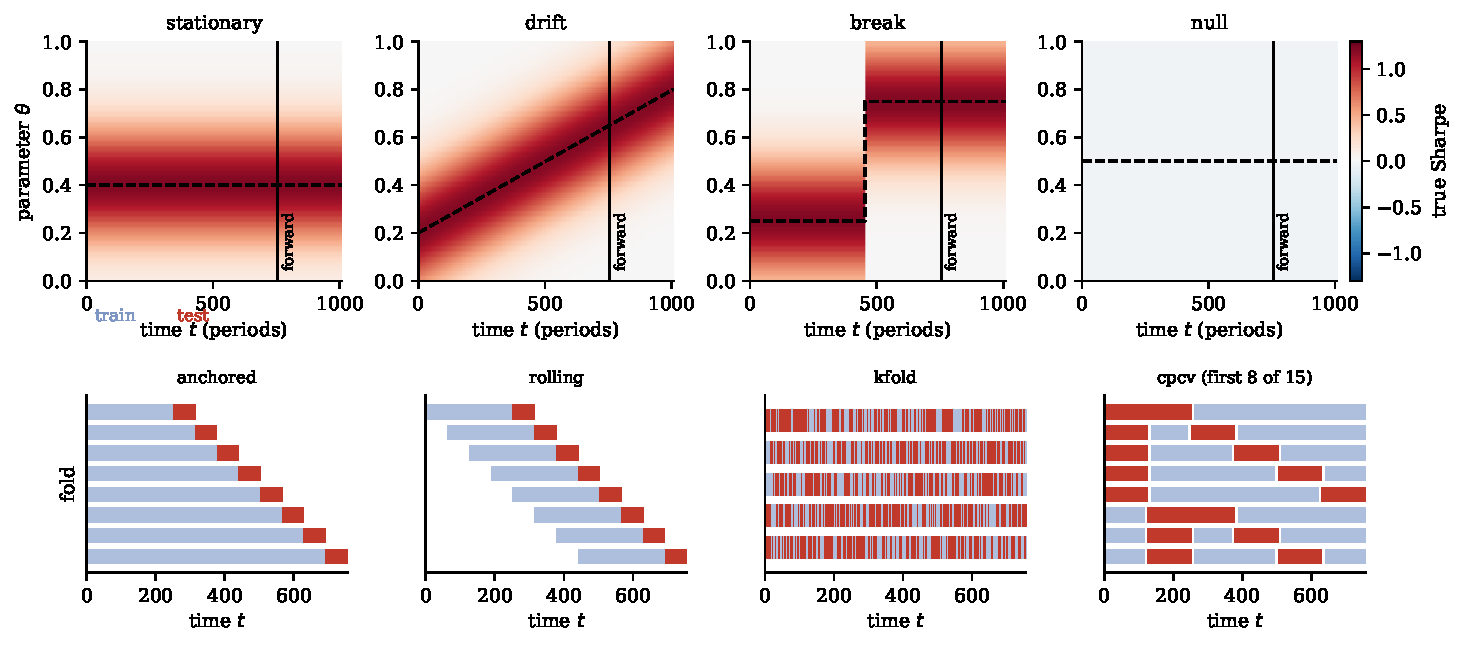
\includegraphics[width=\textwidth]{fig_setup.pdf}
\caption{The generative model and the procedures. \emph{Top:} the true
annualized-Sharpe surface $\srtrue(\theta,t)$ (color) for one canonical
configuration of each regime; the dashed line is the moving optimum $c(t)$
and the vertical line marks the end of the $756$-period history---everything
to its right is the $252$-period forward horizon on which deployments are
judged. \emph{Bottom:} train (blue) and test (red) windows of four procedures
on one $756$-period history with $L_{\mathrm{train}}=252$,
$L_{\mathrm{test}}=63$: anchored WFO (8 expanding folds), rolling WFO (8
fixed-length folds on the same test segments), shuffled $5$-fold (interleaved,
time-blind), and CPCV-lite (first 8 of its 15 group combinations; embargoed
gaps visible at test-group boundaries).}
\label{fig:setup}
\end{figure}

\paragraph{A known, time-varying Sharpe surface.} Each experiment draws a
population surface over the parameter grid,
\begin{equation}
\srtrue(\theta,t) \;=\;
\mathrm{clip}_{\pm 4}\!\left[\, b \;+\; A
\exp\!\left(-\frac{(\theta - c(t))^2}{2 w^2}\right)\right],
\label{eq:surface}
\end{equation}
a Gaussian bump of amplitude $A$ and width $w$ on a floor $b$, whose center
$c(t)$ moves according to the regime: \emph{stationary} ($c(t)=c_0$
throughout), \emph{drift} ($c(t)$ moves linearly from $c_0$ to $c_1$ across
history plus forward horizon), \emph{break} ($c(t)=c_0$ until a sampled break
time inside the history, then jumps to $c_1$), and \emph{null} ($A=0$ with a
non-positive floor: nothing to find). Per-period returns at each grid point
carry a shared market factor,
\begin{equation}
r_t(\theta) \;=\; \frac{\srtrue(\theta,t)}{\sqrt{P}}
\;+\; \sqrt{\phi}\,F_t \;+\; \sqrt{1-\phi}\,\varepsilon_t(\theta),
\qquad P = 252,
\label{eq:returns}
\end{equation}
with $F_t$ and $\varepsilon_t(\theta)$ standard normal, so each column has
unit per-period variance, the population annualized Sharpe at time $t$ equals
$\srtrue(\theta,t)$, and nearby strategies co-move with factor share
$\phi$---the cross-sectional structure walk-forward folds actually face.

\paragraph{Ground truth.} Because the surface is known, the true expected
annualized Sharpe of deploying any $\theta$ over the forward horizon is the
time-average
\begin{equation}
\srfwd(\theta) \;=\; \frac{1}{T_{\mathrm{fwd}}}
\sum_{t=T_{\mathrm{hist}}}^{T_{\mathrm{hist}}+T_{\mathrm{fwd}}-1}
\srtrue(\theta,t)
\label{eq:fwd}
\end{equation}
(the $O(\mathrm{SR}^2/P)$ variance contribution of a moving mean is
negligible at these Sharpe levels). Every procedure is scored on
$\srfwd(\hat\theta_{\mathrm{deploy}})$ of the configuration it would put into
production; a run \emph{deployed a loser} if that value is negative, and its
\emph{regret} is the gap to the forward-optimal
$\max_\theta \srfwd(\theta)$.

\paragraph{Sampled design.} Every constant that affects results is either
disclosed here or recorded per experiment; there are no hidden constants.
Each run independently draws: grid size
$n_\theta \in \{25, 31, 41\}$; history length
$T_{\mathrm{hist}} \in \{504, 756, 1008\}$ with forward horizon
$T_{\mathrm{fwd}} = 252$ fixed; amplitude $A \sim U(0.4, 2.0)$ (zero for
null); width $w \sim U(0.10, 0.35)$; floor $b \sim U(-0.2, 0.2)$ (null:
$b \sim U(-0.10, 0)$); initial center $c_0 \sim U(0.25, 0.75)$; for drift and
break, a shift of magnitude $U(0.2, 0.5)$ in a random direction with $c_1$
clipped to $[0.05, 0.95]$; break time $U(0.3, 0.9)$ as a fraction of the
history; factor share $\phi \sim U(0.05, 0.5)$. Window design follows the
practitioner rules of thumb the recipe itself prescribes: train length a
sampled fraction $\{0.2, 0.3, 0.4, 0.5\}$ of the history, test length $1/4$
or $1/3$ of train (minimum $21$), step equal to the test length (so OOS
segments never overlap, and consecutive rolling train windows overlap by
$67$--$75\%$); the single split holds out a fraction
$\{0.25, 0.30, 0.35\}$; $k$-fold uses $k=5$; CPCV-lite uses $6$ groups,
$2$ test groups, embargo $10$.

\section{Experimental setup}
\label{sec:setup}

The main batch runs $8{,}000$ experiments with regimes cycled for exactly
$2{,}000$ per regime, master seed $101$ spawned into independent per-run
generators. Within each run, \emph{all five procedures see the same simulated
history}, so every cross-procedure comparison is paired. The window-design
sweep holds $T_{\mathrm{hist}} = 756$ fixed and forces the rolling train
length across $\{63, 126, 189, 252, 378, 504\}$ with test length
$\max(21, L_{\mathrm{train}}/3)$, $1{,}500$ runs per cell ($9{,}000$ total;
seed $303$), tracing the fold count from $33$ down to $1$. Everything is
deterministic given the two seeds; no number in this paper depends on
wall-clock or unseeded state.

\section{Results}

\subsection{WFER is informative---and dominated by simpler statistics from
the same folds}
\label{sec:informative}

\begin{table}[t]
\centering
\caption{Diagnostic quality of validation statistics computed from the
rolling walk-forward folds, judged against the true forward Sharpe of the
deployed configuration ($n=8{,}000$; $2{,}000$ per regime). $\rho$ is the
Spearman rank correlation (orientation-aligned: $\theta$-instability enters
with a negative sign); all overall $\rho$ have $p$ below machine precision.
AUC detects ``deployed a loser'' (forward Sharpe $<0$); ``ex-null'' excludes
the no-edge regime. Bold marks the best diagnostic per column (the null
column is statistically indistinguishable from zero throughout).}
\label{tab:diag}
\small
\begin{tabular}{lcccccc@{\hskip 1.6em}c}
\toprule
& \multicolumn{6}{c}{Spearman $\rho$ vs.\ true forward Sharpe} & \\
\cmidrule(lr){2-7}
Diagnostic & overall & station. & drift & break & null & ex-null & AUC \\
\midrule
Normalized WFER       & 0.451 & 0.387 & 0.365 & 0.260 & $0.022$ & 0.338 & 0.743 \\
Raw WFER              & 0.447 & 0.381 & 0.360 & 0.257 & $0.021$ & 0.333 & 0.742 \\
Stitched OOS Sharpe   & 0.529 & 0.469 & 0.435 & 0.320 & $0.017$ & 0.408 & 0.779 \\
OOS $t$-statistic     & \textbf{0.532} & 0.467 & 0.436 & \textbf{0.327} & $0.017$ & 0.410 & \textbf{0.781} \\
IS$\to$OOS rank corr. & 0.516 & \textbf{0.508} & \textbf{0.442} & 0.318 & $0.036$ & \textbf{0.424} & 0.752 \\
Fold win rate         & 0.434 & 0.386 & 0.335 & 0.246 & $-0.012$ & 0.323 & 0.733 \\
$\theta$-instability ($-$) & 0.408 & 0.371 & 0.279 & 0.142 & $-0.004$ & 0.266 & 0.733 \\
\bottomrule
\end{tabular}
\end{table}

Table~\ref{tab:diag} and Figure~\ref{fig:wfer} (left) give the headline
operating characteristics. The normalized WFER is genuinely informative:
Spearman $\rho = 0.451$ against the true forward Sharpe and AUC $0.743$ for
detecting a deployed loser. The folklore is not testing nothing.

But it is never the best statistic on offer. On every column of
Table~\ref{tab:diag} except the noise-level null, both WFER variants are
beaten by at least two of the simpler diagnostics computed from the same
folds: the stitched OOS $t$-statistic ($\rho = 0.532$, AUC $0.781$), the
stitched OOS Sharpe ($\rho = 0.529$, AUC $0.779$), and the IS$\to$OOS rank
correlation ($\rho = 0.516$, and the best per-regime correlations under
stationarity and drift). The mechanism is visible in
\eqref{eq:norm}: the ratio's numerator is essentially the stitched OOS mean,
which carries the forward-relevant information; the denominator is the
selection-\emph{inflated} IS mean, which is noisy and nearly uninformative
about the future, so dividing by it mostly injects noise. Consistent with
this, the two WFER variants rank runs almost identically
($\rho = 0.451$ vs.\ $0.447$): within a run the normalization
\eqref{eq:norm} is a constant factor, so ranking is barely affected---what
the normalization changes is the \emph{location} of the distribution relative
to fixed thresholds, which is exactly where the raw form fails
(Section~\ref{sec:thresholds}).

Three qualifications sharpen the picture. First, quality degrades as the
world becomes less stationary: WFER's per-regime correlation falls from
$0.387$ (stationary) through $0.365$ (drift) to $0.260$ (break), and every
other diagnostic degrades in the same order---validation statistics are most
trustworthy exactly when they are least needed. Second, within the null
regime every diagnostic is uninformative ($|\rho| \le 0.036$, within sampling
noise of zero): once there is no edge, no fold statistic separates
slightly-less-negative from slightly-more-negative deployments. A
substantial part of the headline AUC therefore comes from separating
null from non-null runs: excluding the null regime, WFER's AUC drops from
$0.743$ to $0.685$. Third, the ordering is not an artifact of the rolling
procedure: on anchored folds the picture is the same (WFER $\rho = 0.417$
vs.\ OOS $t$-statistic $0.527$; the IS$\to$OOS rank correlation is anchored's
best at $0.542$).

\begin{figure}[t]
\centering
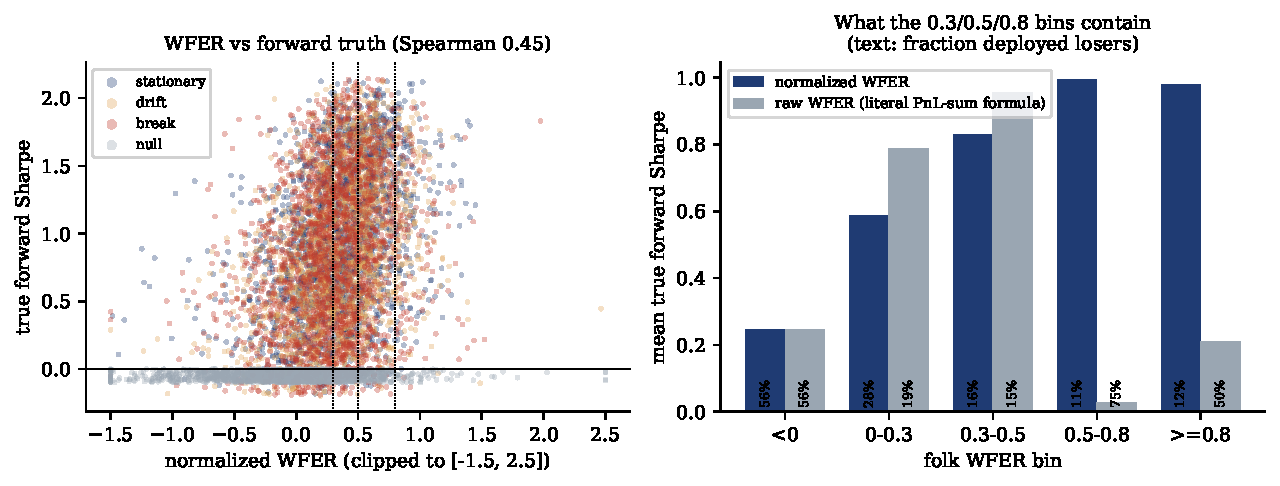
\includegraphics[width=\textwidth]{fig_wfer.pdf}
\caption{\emph{Left:} normalized WFER (rolling WFO) against the true forward
Sharpe of the deployed configuration, all $8{,}000$ runs colored by regime
(WFER clipped to $[-1.5, 2.5]$ for display; Spearman $0.45$). Dotted
verticals mark the folk thresholds $0.3/0.5/0.8$; the gray band at slightly
negative forward Sharpe is the null regime, which spreads across the entire
WFER axis. \emph{Right:} mean true forward Sharpe within each folk bin for
the normalized (dark) and literal raw (gray) WFER; the rotated text gives the
fraction of deployed losers per bin. The raw bars above $0.5$ stand on $4$
and $2$ runs respectively.}
\label{fig:wfer}
\end{figure}

\subsection{The folk thresholds are miscalibrated, and the raw ratio cannot
reach them}
\label{sec:thresholds}

\begin{table}[t]
\centering
\caption{What the folk WFER bins contain (rolling WFO, $n=8{,}000$). The
grading reads $\ge 0.8$ ``excellent,'' $0.5$--$0.8$ ``acceptable,''
$0.3$--$0.5$ ``borderline,'' $<0.3$ ``overfit,'' $<0$ ``unprofitable.''
``loser'' is the share of runs whose deployed forward Sharpe is negative;
``null'' is the share of no-edge-regime runs in the bin. Four runs with
non-positive IS PnL, where the ratio is ill-defined (all null-regime, all
losers), are excluded. The $<0$ rows coincide because the two variants share
the sign of the ratio.}
\label{tab:bins}
\small
\begin{tabular}{lrccc@{\hskip 1.8em}rccc}
\toprule
& \multicolumn{4}{c}{Normalized WFER} & \multicolumn{4}{c}{Raw WFER (literal formula)} \\
\cmidrule(lr){2-5}\cmidrule(lr){6-9}
Bin & $n$ & mean fwd SR & loser & null & $n$ & mean fwd SR & loser & null \\
\midrule
$<0$         & 1947 & 0.246 & 56.5\% & 51.7\% & 1947 & 0.246 & 56.5\% & 51.7\% \\
$0$--$0.3$   & 2324 & 0.588 & 28.4\% & 24.1\% & 5887 & 0.786 & 19.3\% & 16.4\% \\
$0.3$--$0.5$ & 1728 & 0.830 & 16.0\% & 13.4\% &  156 & 0.956 & 15.4\% & 14.1\% \\
$0.5$--$0.8$ & 1543 & 0.994 & 11.4\% & \phantom{0}9.6\% & 4 & 0.029 & 75\% & 75\% \\
$\geq 0.8$   &  454 & 0.980 & 11.9\% & 11.0\% & 2 & 0.212 & 50\% & 50\% \\
\bottomrule
\end{tabular}
\end{table}

Table~\ref{tab:bins} and Figure~\ref{fig:wfer} (right) calibrate the folk
grading against the forward truth, in both readings of the ratio.

\paragraph{Normalized reading: monotone below $0.5$, flat above.} Mean
forward Sharpe rises cleanly through the lower bins ($0.246 \to 0.588 \to
0.830 \to 0.994$) and the loser rate falls ($56.5\% \to 28.4\% \to 16.0\% \to
11.4\%$)---the ratio orders outcomes. But the top grade adds nothing: the
$\ge 0.8$ ``excellent'' bin does \emph{no better} than the $0.5$--$0.8$
``acceptable'' bin ($0.980$ vs.\ $0.994$ mean forward Sharpe; $11.9\%$ vs.\
$11.4\%$ losers). Part of that pooled comparison is regime composition---the
$\ge 0.8$ bin carries slightly more null-regime runs ($11.0\%$ vs.\ $9.6\%$);
excluding the null regime the means remain tied ($1.107$ vs.\ $1.105$) while
the loser-rate ordering reverses and stays insignificant ($1.0\%$ vs.\
$2.0\%$, Fisher $p = 0.21$)---so ``indistinguishable'' is the reading that
survives either composition. And the labels below $0.5$ mislead badly: the
``borderline'' $0.3$--$0.5$ bin averages $+0.830$ forward Sharpe with only a
$16.0\%$ loser rate, and even the ``overfit'' $0$--$0.3$ bin averages
$+0.588$. A desk that discards everything below $0.5$ throws away
$5{,}999$ of our $8{,}000$ runs; the $4{,}052$ of them in the $0$--$0.5$
bins have forward Sharpe averaging $+0.59$ to $+0.83$. The only cut with qualitatively distinct content is the sign: the
$<0$ bin is half null-regime ($51.7\%$) and majority losers ($56.5\%$).

\paragraph{Raw reading: the thresholds are unreachable.} Under the literal
PnL-sum formula \eqref{eq:raw}, $74\%$ of positive-IS runs land in
$0$--$0.3$ and only $6$ of $8{,}000$ runs reach $0.5$ at all. This is
structural, not empirical accident: with IS windows $3$--$4\times$ the OOS
windows, $\wfer_{\mathrm{raw}} \approx (0.25$--$0.33) \times
\wfer_{\mathrm{norm}}$, so reaching $0.5$ requires OOS PnL \emph{per period}
$1.5$--$2\times$ the IS rate---which in practice happens only through an
anomalously small IS denominator. Indeed the six runs that do clear $0.5$
average forward Sharpe $+0.09$ and four of the six are deployed
losers---three in the ``acceptable'' $0.5$--$0.8$ bin (which averages
$+0.029$) and one in the ``excellent'' $\ge 0.8$ bin, a run whose raw ratio
of $4.33$ is the most extreme in the entire sample: under the raw reading, a
high WFER is closer to a danger sign than a seal of quality.
A practitioner who grades the literal ratio against the folk table will
reject essentially everything---or, worse, accept exactly the degenerate
denominators. Any WFER user must therefore state which formula they grade;
the thresholds are only even meaningful per-period normalized.

\subsection{The per-window ratio is ill-conditioned}
\label{sec:illcond}

The folklore also reads efficiency window by window ($O_j/I_j$ per fold).
That ratio explodes whenever a single fold's IS PnL is near zero. We flag a
run as having a \emph{weak-denominator window} if its weakest fold has
$|I_j| < s_j\sqrt{n_j}$, i.e.\ an IS PnL within one standard error of zero
($z_j < 1$). At this one-standard-error threshold the flag catches $21.4\%$ of all runs---$12.3\%$,
$12.7\%$, and $13.5\%$ under stationarity, drift, and break, but $47.3\%$
under the null, exactly where the diagnostic is supposed to protect you. In
flagged runs the median largest per-window $|{\wfer}|$ is $0.88$ versus
$0.43$ in clean runs, and $5.4\%$ of flagged runs contain a window ratio
exceeding $5$ in magnitude (versus $0.0\%$ of clean runs). Loosening the
flag to $z_j < 2$ catches $69.0\%$ of all runs ($96\%$ of null): by the
ordinary standards of statistical significance, most walk-forward runs
contain at least one window whose efficiency reading is built on a
denominator indistinguishable from zero.

The aggregate ratio \eqref{eq:norm} is better protected---only $0.46\%$ of
runs have $|\overline{\mathrm{IS}}|$ within one standard error of zero
($1.6\%$ of null)---but where it happens the statistic collapses: the WFER
interquartile range jumps from $0.49$ (clean) to $2.44$ (flagged), the
correlation with forward truth falls from $0.45$ to $0.08$, and $32\%$ of
flagged runs report $|{\wfer}| > 3$ (versus $0.01\%$ of clean runs). The
practical rule writes itself: never read an efficiency ratio, aggregate or
per window, without first checking that its denominator is statistically
distinguishable from zero.

\subsection{Anchored vs.\ rolling: the folklore direction is right; its
price is not stated}
\label{sec:avr}

\begin{figure}[t]
\centering
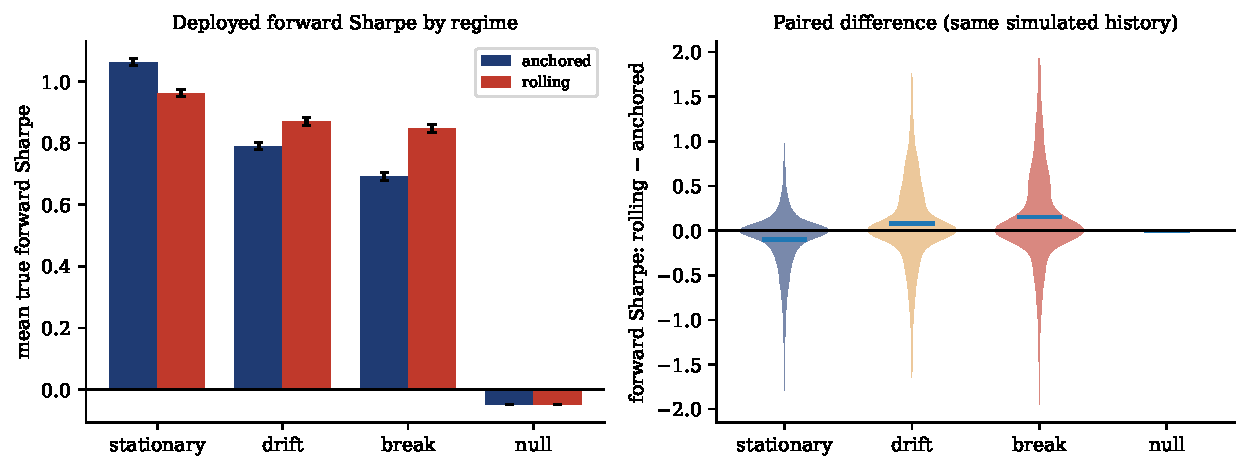
\includegraphics[width=\textwidth]{fig_anchored_vs_rolling.pdf}
\caption{Anchored vs.\ rolling walk-forward, paired on identical histories
and OOS segments ($2{,}000$ runs per regime). \emph{Left:} mean true forward
Sharpe of the deployed configuration by regime, error bars $\pm 1$ SEM.
\emph{Right:} violins of the within-run paired difference (rolling minus
anchored) with the mean marked; under the null the difference is exactly
zero, because the surface is flat in $\theta$ and the deployed parameter is
irrelevant.}
\label{fig:avr}
\end{figure}

Practitioner advice holds that anchored (expanding) windows ``use all the
data'' while rolling windows ``adapt to regime change.'' The paired
comparison in Figure~\ref{fig:avr} confirms the direction and prices it.
Under stationarity, anchored wins: $1.062$ vs.\ $0.962$ mean forward Sharpe,
a paired difference of $-0.100 \pm 0.007$ (Wilcoxon signed-rank with
zero differences discarded, the default convention; ties are $26\%$ of
pairs per regime, and the reported means and standard errors include them;
$p \approx 2\times10^{-39}$). Under drift, rolling wins by $+0.079 \pm
0.009$ ($p \approx 8\times10^{-18}$; rolling wins $44\%$ of paired runs and
loses $30\%$), and under a structural break by $+0.154 \pm 0.011$
($p \approx 5\times10^{-40}$; wins $46\%$, loses $28\%$). Under the null
the two procedures tie exactly. Across our equal-weight regime mix the net
favors rolling, $+0.034 \pm 0.004$ overall ($p \approx 6\times10^{-12}$).

So the folklore's direction survives a controlled test---rolling is
regime-change insurance---but the premium is real and symmetric in size with the
payout: roughly $0.10$ Sharpe forfeited if the world happens to be
stationary, against $0.08$--$0.15$ gained if it drifts or breaks. The choice
is a bet on non-stationarity, not a free robustness upgrade. This echoes,
in a selection-pipeline setting, the econometric result that rolling-window
size should be tuned to the degree of parameter drift
\citep{inoue2017rolling}.

\subsection{Window design matters for the estimate, not the deployment}
\label{sec:window}

\begin{figure}[t]
\centering
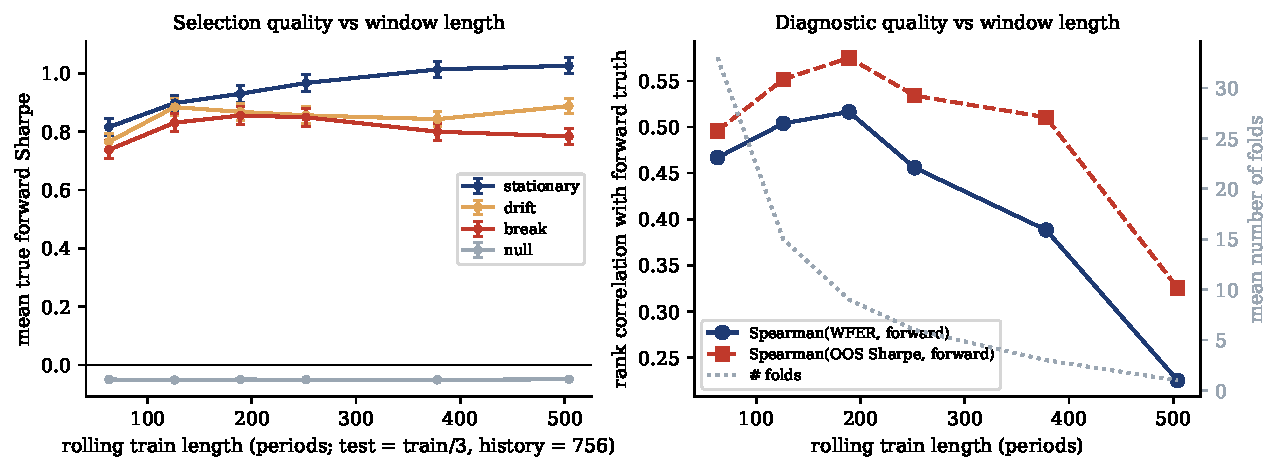
\includegraphics[width=\textwidth]{fig_window_design.pdf}
\caption{The window-design sweep (rolling WFO; history fixed at $756$
periods; test length $= L_{\mathrm{train}}/3$; $1{,}500$ runs per cell).
\emph{Left:} mean true forward Sharpe of the deployed configuration by
regime, $\pm 1$ SEM, across the train-length grid. \emph{Right:} Spearman
correlation of the normalized WFER (solid) and the stitched OOS Sharpe
(dashed) with the forward truth; the dotted gray curve (right axis) is the
mean number of folds, falling from $33$ at $L_{\mathrm{train}}=63$ to $1$ at
$504$. Both diagnostics peak near nine folds and collapse at one; the OOS
Sharpe dominates WFER at every train length.}
\label{fig:window}
\end{figure}

The sweep (Figure~\ref{fig:window}) separates two questions the folklore
runs together: does window design change \emph{what you deploy}, and does it
change \emph{what you know about it}?

\paragraph{Deployment is forgiving.} Mean deployed forward Sharpe is
$0.567$ at $L_{\mathrm{train}} = 63$ and then essentially flat from $126$
up: $0.640$, $0.651$, $0.655$, $0.651$, $0.662$ across
$\{126, 189, 252, 378, 504\}$. Only a train window too short to estimate the
surface ($63$ periods, one calendar quarter) measurably hurts. Beneath the
flat aggregate there is mild regime texture that the folklore's
``shorter adapts faster'' intuition only partly anticipates: stationary runs
improve monotonically with train length ($0.815 \to 1.026$), break runs peak
at $189$ ($0.855$) and fade to $0.784$ by $504$, and drift runs are flat
within noise ($0.84$--$0.89$) for $L_{\mathrm{train}} \ge 126$.

\paragraph{The estimate is not.} The diagnostic quality of the same folds
moves a lot. The WFER--forward rank correlation rises from $0.467$
($33$ folds of a noisy-short window) to a peak of $0.516$ at
$L_{\mathrm{train}} = 189$ (nine folds), then collapses as folds disappear:
$0.456$ (six), $0.388$ (three), and $0.225$ at the
single-fold corner---which is exactly the single train/test split that much
practice still defaults to. The stitched OOS Sharpe traces the same arc ($0.496 \to 0.575
\to 0.325$) and dominates WFER at every train length. The RMSE of the
stitched OOS Sharpe as an estimator of the forward Sharpe rises
from ${\approx}0.72$--$0.73$ at many folds to $1.33$ at one fold (the rise
is essentially monotone, with a $0.003$ dip between the two longest
many-fold settings), while its
\emph{bias} stays below $0.02$ in magnitude in every cell: fold-stitching
buys variance reduction, not bias correction. The actionable summary: pick
the train window long enough to learn the surface (${\ge}126$ periods here),
then cut the rest of the history into as many non-overlapping OOS segments
as that allows---the deployment will not care, and every diagnostic will.

\subsection{Procedure ranking: rolling deploys best; shuffled $k$-fold
flatters most; CPCV-lite ranks best}
\label{sec:ranking}

\begin{table}[t]
\centering
\caption{The five procedures on the same $8{,}000$ histories. Left block:
mean true forward Sharpe of the deployed configuration, overall and per
regime (under the null all procedures earn the same $-0.049$: the surface is
flat in $\theta$, so the deployed parameter is irrelevant). Right block: the
procedure's own validation estimate (stitched OOS Sharpe)---signed bias
(estimate minus forward truth; overall, drift, break) and Spearman
correlation with the forward truth. Anchored and CPCV-lite deploy the same
configuration (full-history argmax) by construction, hence identical forward
columns. Bold marks the best per column.}
\label{tab:proc}
\small
\begin{tabular}{lcccc@{\hskip 1.6em}cccc}
\toprule
& \multicolumn{4}{c}{True forward Sharpe (deployed)} &
\multicolumn{4}{c}{Validation estimate} \\
\cmidrule(lr){2-5}\cmidrule(lr){6-9}
Procedure & overall & station. & drift & break & bias & bias$_{\text{drift}}$ & bias$_{\text{break}}$ & $\rho$(est, fwd) \\
\midrule
Single split      & 0.558 & 1.030 & 0.702 & 0.551 & $+0.073$ & $+0.212$ & $+0.103$ & 0.477 \\
Anchored WFO      & 0.624 & 1.062 & 0.790 & 0.692 & $+0.048$ & $+0.149$ & $+0.071$ & 0.524 \\
Rolling WFO       & \textbf{0.657} & 0.962 & \textbf{0.869} & \textbf{0.846} & $\mathbf{+0.013}$ & $\mathbf{+0.060}$ & $\mathbf{-0.034}$ & 0.529 \\
Shuffled $k$-fold & 0.623 & \textbf{1.066} & 0.788 & 0.688 & $+0.083$ & $+0.191$ & $+0.147$ & 0.541 \\
CPCV-lite         & 0.624 & 1.062 & 0.790 & 0.692 & $+0.049$ & $+0.155$ & $+0.079$ & \textbf{0.636} \\
\bottomrule
\end{tabular}
\end{table}

Table~\ref{tab:proc} ranks the procedures on both jobs a validation scheme
performs: choosing what to deploy, and estimating how it will do.

\paragraph{Deployment.} Rolling WFO deploys best overall ($0.657$; mean
regret against the forward-oracle $0.226$), entirely through its advantage
under drift and breaks; under stationarity it pays the recency price of
Section~\ref{sec:avr}. Anchored, CPCV-lite, and shuffled $k$-fold form a
cluster near $0.623$--$0.624$---unsurprisingly, since all three effectively
deploy a full-history selection ($k$-fold's CV-mean argmax lands almost
exactly where the full-history argmax does). The single split is clearly
worst ($0.558$; regret $0.325$): it selects on only the first
$65$--$75\%$ of the history, and under drift or break the discarded recent
data is precisely the most relevant.

\paragraph{Estimates.} The shuffled $k$-fold is the most optimistic estimator
overall ($+0.083$ Sharpe bias), and its failure is regime-specific in the
way \citet{lopezdeprado2018advances} and \citet{cerqueira2020evaluating}
would predict: essentially unbiased under stationarity ($-0.006$, consistent
with the validity result of \citet{bergmeir2018note} for this serially
independent DGP), but $+0.191$ under drift and $+0.147$ under break, because
interleaved test folds let the procedure train on the future of the very
points it tests. Notably, the single split's estimate is even \emph{worse}
under drift ($+0.212$): one early-selected configuration, one late test
window, and a forward horizon that keeps moving. Rolling is the least biased
overall ($+0.013$), though this is partly cancellation ($+0.060$ drift,
$-0.034$ break, $+0.002$ stationary). And a sobering regularity cuts across
all five procedures: under drift every bias is positive---when the optimum
moves, decay continues into the deployment horizon, so even a perfectly
honest OOS estimate is a backcast, not a forecast.

\paragraph{Ranking quality.} As a \emph{ranking} signal across runs,
CPCV-lite's estimate is the clear winner ($\rho = 0.636$ vs.\
$0.524$--$0.541$ for everything else): averaging $15$ combinatorial paths
stabilizes the estimate even in a DGP with no label leakage to purge,
supporting the multiple-paths argument for CPCV
\citep{lopezdeprado2018advances} on grounds independent of purging. The
single split is the weakest ranker ($0.477$) as well as the weakest
deployer---the worst of both worlds.

\section{Discussion}
\label{sec:discussion}

\paragraph{If you run walk-forward, you already have something better than
WFER.} The ratio's numerator---stitched OOS performance---is where the
information lives; its denominator adds selection-biased noise and a
divide-by-near-zero failure mode. On every regime with an edge, the stitched
OOS $t$-statistic and Sharpe dominate WFER on both ranking and
loser-detection, at zero additional computational cost. The IS$\to$OOS rank
correlation is a strong complement (best under stationarity and drift, and
for anchored folds), because it uses the whole $\theta$-cross-section per
fold instead of one selected point. If a ratio must be reported, it should be
the per-period normalized form \eqref{eq:norm}, accompanied by a check that
the IS denominator is statistically distinguishable from zero---a check that
fails somewhere in most runs at conventional significance
(Section~\ref{sec:illcond}).

\paragraph{Retire the grading table.} In its only coherent (normalized)
reading, the folk grading gets one thing right---the ordering below
$0.5$---and both of its labels wrong: the ``excellent'' grade above $0.8$
contains nothing the ``acceptable'' bin does not, and the
``borderline/overfit'' zone below $0.5$ averages solidly positive forward
performance in our world. The literal raw-PnL form cannot reach the
thresholds at all, and the six runs that do reach them are dominated by
degenerate denominators. The defensible uses of WFER are relative (ranking
candidate configurations within a shop) and sign-based (a negative ratio is a
genuine red flag: $56.5\%$ losers, half of them null-regime). Absolute
grades imported from folklore transfer neither across window designs (raw
vs.\ normalized differ by a factor of $3$--$4$ here by construction) nor, on
this evidence, across the $0.5$ line where the bins stop separating.

\paragraph{Window folklore, repriced.} Anchored-vs.-rolling should be
presented as a bet, not a best practice: rolling buys $0.08$--$0.15$ of
forward Sharpe under drift and breaks at a premium of $0.10$ under
stationarity. Window length is the reverse: it barely moves the deployment
(above a minimum train length) but strongly moves how much the validation
\emph{tells} you, peaking near nine folds in our setting and collapsing at
the single-split corner. The common default of one IS/OOS split is
quantifiably the worst choice on both axes. And the $k$-fold warning for
finance deserves its precise form: with serially independent returns the
scheme's estimate is fine under stationarity; what kills it is
non-stationarity, where it trains on the future and overstates forward
Sharpe by $0.15$--$0.19$---while \emph{deploying} essentially the same
configuration as anchored WFO. The danger is the number it reports, not the
parameter it picks.

\section{Limitations}
\label{sec:limitations}

Our returns are Gaussian and serially independent given the surface, with a
single constant-share market factor; real returns have fat tails, volatility
clustering, and dependence that would degrade all diagnostics further and
could re-order them---in particular, CPCV-lite's embargo does no real work
here because there is no label overlap to purge, so our CPCV result speaks
to its multiple-paths averaging, not its purging. The strategy family is
one-dimensional with a single Gaussian bump; interacting parameters and
multimodal surfaces (studied in a sibling paper on plateau heuristics) are
out of scope. The selection rule is everywhere the argmax of train-window
Sharpe; regularized or shape-aware selection would change both deployments
and diagnostics. Our regimes are stylized (linear drift, single break, fixed
$252$-period forward horizon), the surface amplitude range
($0.4$--$2.0$ annualized Sharpe) is generous, and lower true edges would
lower every correlation in Table~\ref{tab:diag}. The bin-calibration
findings also depend on the surface geometry: in worlds with optima far
sharper than our sampled widths ($0.10$--$0.35$), the top WFER grade can
begin to separate from the next one, so the ``flat above $0.5$'' result
should be read within the disclosed width range. The thresholds are
evaluated as bins over a heterogeneous design mix, not as decision policies
with explicit costs; and our normalized WFER is one disclosed reading of
``annualized OOS over annualized IS''---other normalizations (per-trade,
risk-adjusted) circulate. Finally, we model no transaction costs and no
re-optimization during the forward horizon, which a live walk-forward
deployment would perform.

\section{Conclusion}

We gave walk-forward validation's acceptance statistic its first controlled
test against a known ground truth. The walk-forward efficiency ratio is
informative but strictly redundant: every job it does is done better by the
stitched OOS $t$-statistic, OOS Sharpe, or IS$\to$OOS rank correlation
computed from the same folds, and its distinguishing operation---dividing by
in-sample PnL---contributes noise, a degenerate-denominator failure mode
affecting one run in five (and half of the no-edge runs), and a units problem
that makes the popular thresholds unreachable in their literal raw-PnL form
($6$ of $8{,}000$ runs). The folk grading is miscalibrated even in its
coherent normalized reading: nothing separates ``excellent'' from
``acceptable,'' and the ``overfit'' zone averages $+0.59$ to $+0.83$ forward
Sharpe. The window folklore fares better: rolling windows do beat anchored
under drift and breaks (and cost $0.10$ under stationarity), window length
matters chiefly through the number of folds and hence the quality of the
estimate, and walk-forward's forward-chained structure does discipline the
estimate relative to a shuffled $k$-fold---whose optimism under
non-stationarity we quantify at $+0.15$ to $+0.19$ Sharpe. Validate with
walk-forward, by all means; read its OOS track record directly, guard every
denominator, and leave the $0.8/0.5/0.3$ table behind.

\paragraph{Reproducibility.} All experiments are deterministic given the
released seeds ($101$ for the main batch, $303$ for the window sweep). A
single command (\texttt{python scripts/run\_all.py}) regenerates every
result, \texttt{python -m wfo\_experiments.figures} regenerates every
figure, and \texttt{scripts/check\_paper\_numbers.py} verifies that every
number quoted in this paper matches the generated results to rounding. The
generative model, the five procedures, the diagnostics, and the analysis are
provided as an open-source package.

\small
\bibliographystyle{plainnat}
\bibliography{refs}

\end{document}
